
\documentclass{scrreprt}

%
%  Packages
%

\usepackage[pdfborder={0 0 0}]{hyperref} % No we dont want our links to have stupid colors.
\usepackage[english]{babel}
\usepackage{booktabs}
\usepackage{graphicx}
\usepackage[nounderscore]{syntax}
\usepackage{listings}
\usepackage{float}
\usepackage{mips}
\usepackage{verbatim}

\usepackage{bold-extra}

\newcommand{\code}[1]{\texttt{#1}}

\lstset{
         basicstyle=\footnotesize\ttfamily,
         numbers=left,               
         numberstyle=\tiny,                      
         numbersep=8pt,              
         tabsize=2,        
         breaklines=true,            
         keywordstyle=\textbf,
         stringstyle=\ttfamily,
         showspaces=false,
         showtabs=false,
         xleftmargin=17pt,
         showstringspaces=false, 
}



%
%  Front page stuff
%

\title{A peephole optimiser for SimpleScalar DLX assembly code}
\author{J. Stork, L. Swartsenburg and J. Zuiddam}


%
%  Content
%

\begin{document}
\maketitle

\tableofcontents

\chapter{Introduction}
\label{sec:introduction}
In this report, we describe our implementation of a ``peephole'' code optimiser.
Such an optimiser scans and performs transformations on a ``peephole'' of source
code, i.e.\ on a sliding sub-sequence of instructions in that source code. The
function of a peephole optimiser is to improve a computer programme at
compile-time by reducing its typical resource footprint in terms of CPU time,
memory size, or both CPU and memory usage. The peephole optimiser assignment
concludes our undergraduate course on compilers at the University of Amsterdam.



\chapter{Implementation}
In this section we discuss our peephole optimiser. We first give an overview of the general design of the optimiser. We then discuss the implementation of the parts of the optimiser.
\section{Design}
\label{sec:design}
A peephole optimiser rewrites assembly code to make ik more efficient, in terms of processor cycles and memory usage. The general procedure is:
\begin{enumerate}
\item assembly parsing;
\item division in basic blocks;
\item optimisation;
\item assembly generation.
\end{enumerate}
See also figure~\ref{fig:diagram}. We discuss stages 1 and 4 first and then stage 2 and stage 3.

\begin{figure}[h!]
\centering
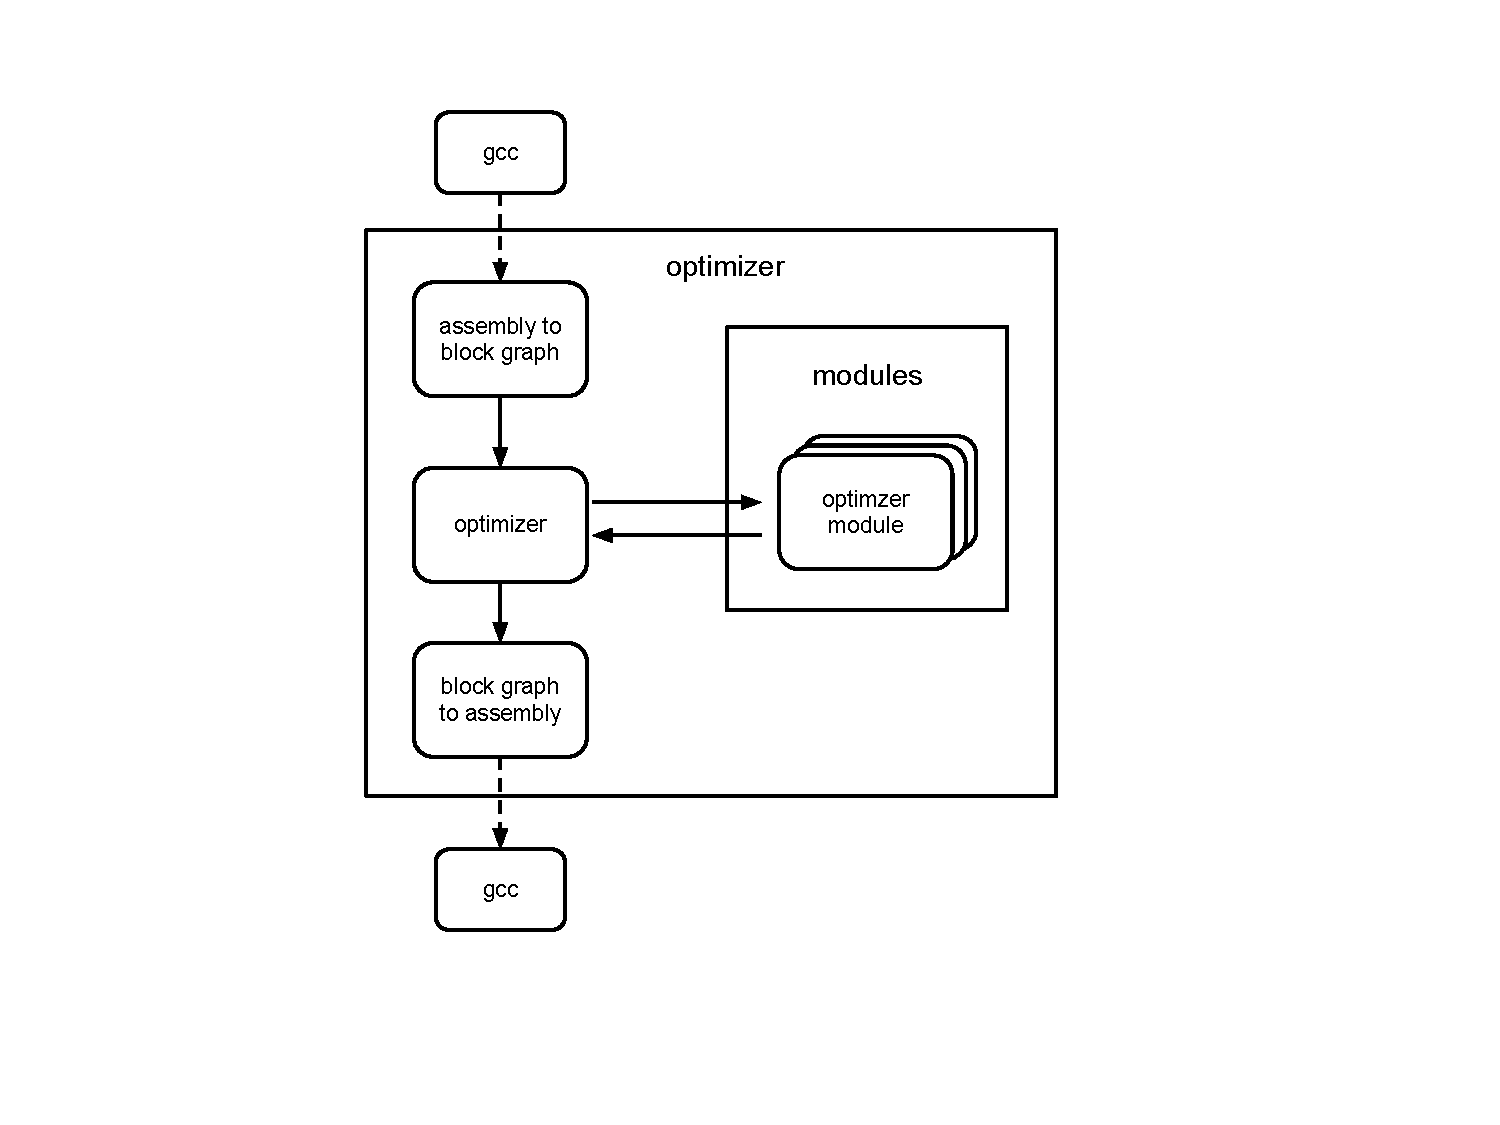
\includegraphics[viewport= 170 90 510 490, clip=true]{diagram}
\caption{Optimiser design diagram.}
\label{fig:diagram}
\end{figure}


\subsection*{Assembly parsing and generation}
As processing an assembly program in the form of a set of text strings is difficult, the optimiser translates the input to an intermediate representation (ir) in the first stage. This translation is called \emph{parsing}. The resulting representation is a list of Python objects, where each object represents an assembly instruction. After optimising, the resulting intermediate representation is translated back to assembly code. Ideally, when no optimisation is done between parsing assembly and regenerating assembly, the composite function $4\circ 1$ is the identity function on the set of all assembly programs. (In our implementation, comments are left out in some cases, and spacing is sometimes changed.)

\subsection*{Division in basic blocks}
Before optimising, the ir is split in \emph{basic blocks}. A basic block is a set of consecutive instructions having a single entry point and a single exit point. By definition, only the first line $i_1$ of a basic block $(i_1, \ldots, i_k)$ can be a jump destination and only the last line $i_k$ can be a jump. Therefore, the execution flow is always $i_1\rightarrow i_2 \rightarrow \cdots \rightarrow i_k$. This property reduces the complexity of doing certain optimisations on instructions in a basic block.

Basic blocks can in turn be divided in functions, linked together by \emph{jump and link} instructions, \code{jal}. We call the set of instructions in a function a \emph{frame}. Frames have a single entry point (on frame level), but not necessarily a single exit point.

\subsection*{Optimisation}
In the optimisation stage, the original intermediate representation $A$ is transformed into a new ir $B$, such that
\begin{enumerate}
\item the new representation $B$ has the same \emph{meaning} as $A$, in terms of program output and behaviour;
\item the execution of the program corresponding to $B$ takes less processor cycles and uses less memory.
\end{enumerate}

\subsubsection*{Optimisation types}
There are two main types of optimisations: graph level optimisations and block level optimisations. 
Our optimiser performs the following graph optimisations:
\begin{itemize}
\item unused block removal,
\item graph flattening, and
\item global branch optimisations,
\end{itemize}
and the following block optimisations:
\begin{itemize}
\item dead code elimination,
\item copy propagation, and
\item constant folding.
\end{itemize}
The optimisations are explained in the implementation sections that follow.


\subsubsection*{Scheduling}
As there are multiple optimisations to apply and a single optimisation may be applied multiple times, we must decide how to schedule them. In this sections we will regard graph and block optimisations as functions on the set of control flow graphs and ir blocks, respectively.

Let $f$ be an optimisation on blocks. It is possible that an application of $f$ on a block $B$ yields a block that in turn can be optimised. That is, applying $f$ on $f(B)$ will yield a different result than $f(B)$. Therefore, $f$ is applied to $B$ until the result is constant, i.e. $n$ times, with $$f^{(n)}(B) = f^{(n-1)}(B).$$ We denote the function that applies $f$ until the result is stable with $f^*$. Note that $f^{(k)}(B)$ for some $k$ need not necessarily be more efficient than $B$ to be useful, because other optimisations can take advantage of the changes made.

Let $f$ and $g$ be two different optimisations on blocks. We could apply $f^*$ to a block $B$ and then $g^*$. But, as $f^*$ and $g^*$ may be mutually beneficial, the composite application $g^* \circ f^*$ must be repeated until the result is constant.

The same properties hold when $f$ and $g$ are graph level optimisations, \emph{mutatis mutandis}. We could even mix graph and block optimisations, where block optimisations are applied to all blocks in the graph concerned. Let $F_1, \ldots, F_m$ be such optimisations. Then, every optimisation must be repeated until constant, which we called $F_i^*$, and the composite optimisation must also be repeated until constant, giving $${(F_m^* \circ \cdots \circ F_1^*)}^*.$$ This is the general scheduling recipe.

We did not consider the order of applying optimisations. A particular order could be optimal. However, as the composite optimisation is repeated until the result is constant, the precise order probably is not decisive.




\section{Instruction parsing}
\label{sec:parsing}
\lstset{ %
language=Python,                % the language of the code
}

For instruction parsing we use Python Lex-Yacc (PLY), an implementation of Lex and Yacc for Python. The Lex part of PLY splits the source in \emph{tokens}, e.g. a \verb!COMMENT!, or a comma. These tokens are passed to Yacc, which finds hierarchical structure in them. When Yacc recognizes a certain pattern, a corresponding action is taken.

\subsection{Lex}

Our lexer splits the source in six tokens: \verb!COMMENT! for comments, \verb!RAW! for compiler directives (lines starting with a dot), \verb!HEX! for hexadecimal values, \verb!INT! for integer values (unsigned), \verb!ID! for label names and instruction names, and \verb!REGISTER! for register identifiers (\verb!$1!, \verb!$2!, etc.)
The following regular expressions specify the tokens.
\begin{quote}
\begin{verbatim}
COMMENT  : #.*
RAW      : \..+
HEX      : 0x[0-9a-f]+
INT      : [0-9]+
ID       : ($L){0,1}[_a-zA-Z0-9][_a-zA-Z0-9\.]*
REGISTER : $[a-z0-9]+
\end{verbatim}
\end{quote}
In addition, we consider the characters `\verb!,!', `\verb!(!', `\verb!)!', `\verb!:!', `\verb!.!', `\verb!+!', and `\verb!-!' as individual tokens, called \emph{literals}.

\subsection{Yacc}
We specified the structure of the assembly language according to the following grammar rules.

\begin{grammar}
<expr> := <raw>
\alt <label>
\alt <comment>
\alt <instr>
\alt <instr> <comment>

<raw> := \verb!RAW!

<label> := \verb!ID! `:'

<comment> := \verb!COMMENT!

<instr> := \verb!ID!
\alt \verb!ID! <arg>
\alt \verb!ID! <arg> `,' <arg>
\alt \verb!ID! <arg> `,' <arg> `,' <arg>

<arg> := <int>
\alt <hex>
\alt <register>
\alt \verb!ID!
\alt \verb!ID! `+' <arg>
\alt \verb!ID! `-' <arg>
\alt <int> `(' <register> `)'
\alt \verb!ID!  `(' <register> `)'

<int> := \verb!INT!
\alt `-' \verb!INT!

<hex> := \verb!HEX!

<register> := \verb!REGISTER!
\end{grammar}

Each expression is stored in a Python object of type \verb!Raw!, \verb!Label!, \verb!Comment!, \verb!Instr! or \verb!Register!.

\subsection{Registers}
To perform dataflow analysis and liveness analysis, we need to parse each 
instruction to determine which registers are set and which registers are used. 
All instructions have a different format, so they need to be parsed seperatly. 
This process is done in the \code{parse\_instr} module. When we run \code{parse\_instr.parse},
it parses each Instr object from the \code{ir} module and sets the register that the
instructoin writes to, the registers that it needs, the offset for writing to 
memory, and immidiate values. An example:
\begin{lstlisting}
if ins.instr == 'add':  
    if len(ins.args) == 3:
        self.gen = [ins.args[0]]
        if self.is_reg(ins.args[2]):
            self.need = [ins.args[1], ins.args[2]]
        else: 
            self.need = [ins.args[1]]
            self.ival = ins.args[2]
    else:
        raise Exception("Invalid number of args for ins: ", ins.instr)   
\end{lstlisting}


\section{Division of instructions into basic blocks}
\label{sec:splitting}
As mentioned in section~\ref{sec:design} we split the source code on two levels.
\begin{itemize}
\item The code is split in functions.
\item Each function is split in \emph{basic blocks}.
\end{itemize}

The blocks of each frame are stored in a \emph{control flow graph} (cfg). The edges in this graph correspond to possible branches.

Splitting in blocks is implemented in \code{cfg.py}.

\section{Control Flow Graph optimisations}
\label{sec:graph}
\lstset{ %
language=[mips]Assembler,         % the language of the code
basicstyle=\footnotesize,         % the size of the fonts that are used for the code
backgroundcolor=\color{white},    % choose the background color. You must add \usepackage{color}
showspaces=false,                 % show spaces adding particular underscores
showstringspaces=false,           % underline spaces within strings
showtabs=false,                   % show tabs within strings adding particular underscores
frame=single,                     % adds a frame around the code
tabsize=2,                        % sets default tabsize to 2 spaces
captionpos=b,                     % sets the caption-position to bottom
breaklines=true,                  % sets automatic line breaking
breakatwhitespace=false,          % sets if automatic breaks should only happen at whitespace
}
In the section \ref{sec:splitting} the code is divided in frames and after
that in basic blocks. It is also possible to create a graph from the whole code.
If this is done, it is possible to perform optimalisations on the graph. We 
implemented two optimalisations in the module optimise\_tree.
\subsubsection{Remove not used}
A program has only one entry point: the beginning of the instruction list. The 
first block should be the only block with no incoming edges. If there are more
blocks with no incoming edges, then these can be removed since they will never 
be reached. The blocks with no edges are the blocks that are between a jump
and a label in the assembly code:
\begin{lstlisting}
    addu    $2,$3,4
    j       $L6
|   bne     $2,$0,$L5
|   mtc1    $2,$f0
|   lw      $31,52($sp)
|   lw      $fp,48($sp)
|   .loc    1 5
|   .ent    main        
$L6:
    div.d   $f0,$f0,$f2	
\end{lstlisting}
In this case, there are two lines that contain raw code. This code is used by
gcc and can therefore not be removed. So we keep \texttt{.loc} and \texttt{.end} 
and we remove \texttt{bne}, \texttt{mtc1} and the \texttt{lw} instructions. If
the raw types wouldn't be there, the jump would now be optimised in 
\ref{sec:global}.
\subsubsection{Flatten the graph}
For all blocks that have one incoming edge (now: "block two") and a block on the 
other side that has only one outgoing edge (now: "block one"), the blocks can 
be placed after eachother in the code. This can work out well when the only 
edge to a block is caused by a jump. This jump will become redundant if the 
blocks are repositioned. We implented this by appending all instructions from 
block two to the instructions from block one and by removing block two as a 
block object. 
\subsubsection{Result}
We made a code that generates a diagram from our graph when the verbosity level
is three. We generate a diagram image before and 
after optimalisation. The result is displayed for pi.s in a \ref{fig:before} 
and \ref{fig:after}.
\begin{figure}[H]
\centering
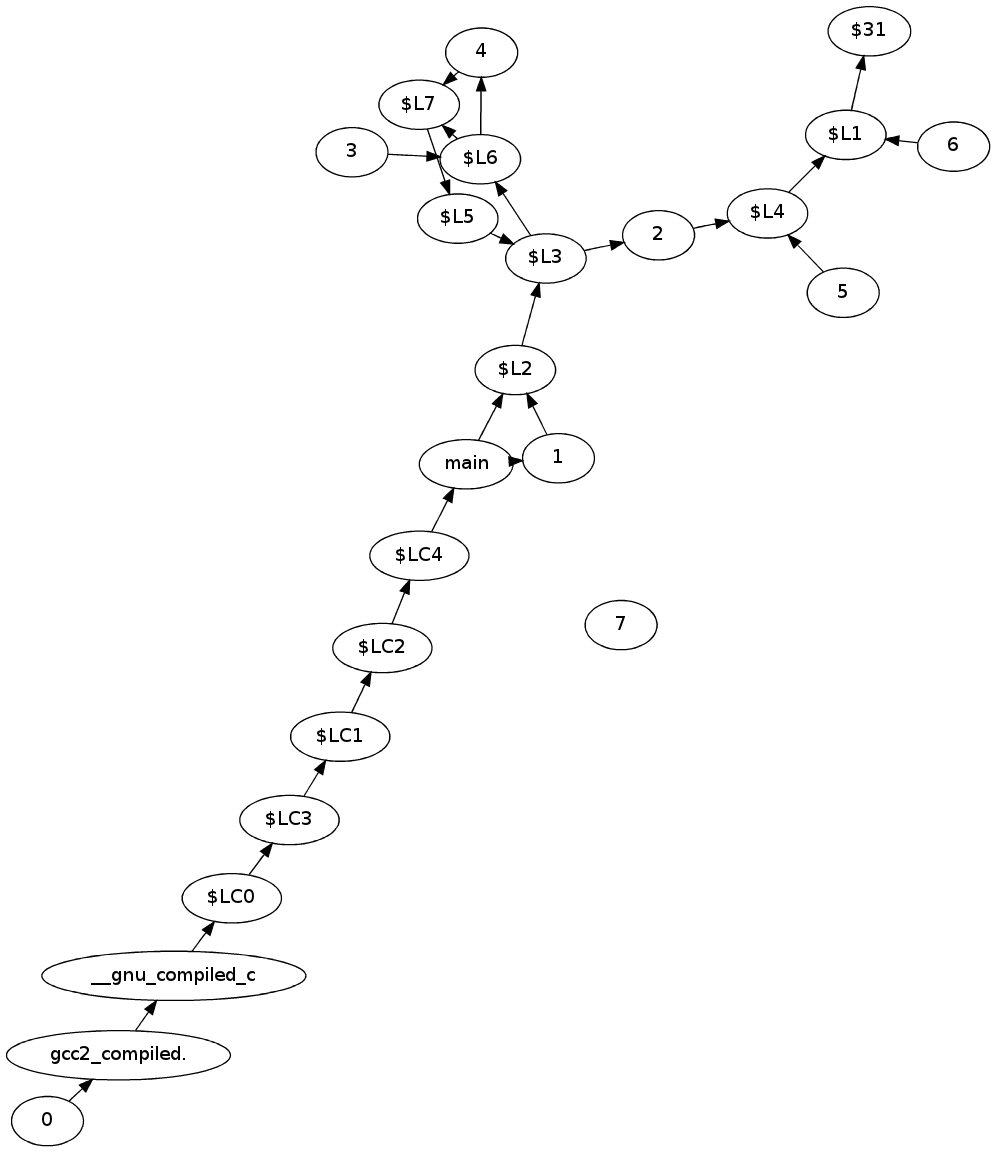
\includegraphics[scale=0.2]{images/before}
\caption{CFG for pi.s before optimalisation}
\label{fig:before}
\end{figure}
\begin{figure}[H]
\centering
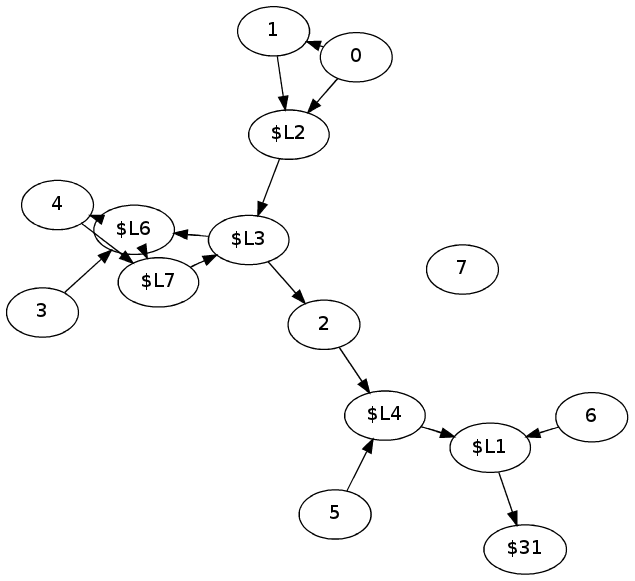
\includegraphics[scale=0.2]{images/after}
\caption{CFG for pi.s after optimalisation}
\label{fig:after}
\end{figure}
After the graph optimalisations we need to perform global jump optimalisations
to actually gain performance.



\section{Global branch optimisations}
\label{sec:global}
\lstset{ %
language=[mips]Assembler,         % the language of the code
}

The flat module contains five different optimalisation functions that remove
redundant code on a global basis. In this subsection we will elaborate on those 
functions. These functions perform better when comments are removed so there is
a function that removes all comments from the code. We decided to not lose 
information in the assembly code.
\subsubsection{Jump - code - Label}
When there is a jump, every code that is between the jump and the label is 
never reached. Thus: the instruction between a jump and a label can be removed.
This function probably will not speed up the code, but can reduce
lines in the assembly code.
Example:
\begin{lstlisting}
    addu    $2,$3,4
    lw      $3,60($fp)
    j       $L4
    mtc1    $2,$f0
    div.d   $f0,$f0,$f2	
$L6:
    jal     random 
\end{lstlisting}
Becomes:
\begin{lstlisting}
    addu    $2,$3,4
    lw      $3,60($fp)
    j       $L4
$L6:
    jal	    random 
\end{lstlisting}
\subsubsection{Label - Label}
When two labels placed directly after eachother, one of the two is redundant.
The second label is removed and each jump in the code that jumps to the second 
label is changed to jump to the first label. This function can reduce lines and
basicblocks for later on in optimalisation. In combination with the jump 
optimalisation "useless branches" this can potentially speed up the program.
Example:
\begin{lstlisting}
    addu    $2,$3,4
    lw      $3,60($fp)
    bne     $2,$0,$L6
    mtc1    $2,$f0
    div.d   $f0,$f0,$f2	
$L5:
$L6:
    jal	    random 
\end{lstlisting}
Becomes:
\begin{lstlisting}
    addu    $2,$3,4
    lw      $3,60($fp)
    bne     $2,$0,$L5
    mtc1    $2,$f0
    div.d   $f0,$f0,$f2	
$L5:
    jal     random 
\end{lstlisting}
\subsubsection{Label - Jump}
If a jump comes directly after a label, both are redundant. We can remove both
lines and adjust all control instructions that point to the label so that they
point to the label the jump was pointing to. If this situation occurs, two
lines of assembly can be removed and the program is optimised by removing one 
jump.
Example:
\begin{lstlisting}
    addu    $2,$3,4
    bne     $2,$0,$L5
    mtc1    $2,$f0
$L5:
    j       $L8
$L6:
    div.d   $f0,$f0,$f2	
\end{lstlisting}
Becomes:
\begin{lstlisting}
    addu    $2,$3,4
    bne     $2,$0,$L8
    mtc1    $2,$f0
$L6:
    div.d   $f0,$f0,$f2	
\end{lstlisting}
\subsubsection{Useless branch/jump}
If a control function jumps to a label that comes directly after the jump/branch
, the instruction can be removed. This results in a smaller assembly file and
a faster program.
Example:
\begin{lstlisting}
    addu    $2,$3,4
    bne     $2,$0,$L6
$L6:
    div.d   $f0,$f0,$f2	
\end{lstlisting}
Becomes:
\begin{lstlisting}
    addu    $2,$3,4
$L6:
    div.d   $f0,$f0,$f2	
\end{lstlisting}
\subsubsection{Branch - Jump - Label}
This function removes a jump when we find a branch - jump - label
combination where the branch points to the label. We can optimise this
by negating the brench, making it point to the jump adres and removing the
label. This results in a smaller assembly file and
a faster program.
Example:
\begin{lstlisting}
    slt     $2,$2,$3
    bne     $2,$0,$L6
    j       $L4
$L6:
    jal     random
\end{lstlisting}
Becomes:
\begin{lstlisting}
    slt     $2,$2,$3
    beq     $2,$0,$L4
$L6:
    jal     random
\end{lstlisting}


\section{Peephole optimisation on basic blocks}
\label{sec:peephole}
This section describes the framework for the basic-block optimisers in our
peephole optimiser, before discussing the different optimisers as we have
implemented them.\\

In order to focus our optimisation efforts, we drew up a ranking of instructions
in the benchmark suite (see table~\ref{tab:irank} on page~\pageref{tab:irank})
using an instruction ranker we made for the purpose (source in appendix
section~\ref{sec:ranker} on page~\pageref{sec:ranker}). Based on the incidence
of certain instructions, and on the fact that we wished to develop basic-block
optimisers in parallel with both global and ``advanced'' (dataflow and liveness
analysis based) optimisations, we decided to focus on: copy propagation; dead
code removal; constant folding; and algebraic transformations.
Subsections~\ref{sub:copyprop} through~\ref{sub:algebratrans} below describe
these basic-block optimisations before discussing the choices and considerations
involved in their respective implementations.\\

\begin{table}[ht]
\centering
\begin{tabular}{l l l l l l}
\toprule
opcode  &occurences &opcode  &occurences &opcode &occurences \\
\midrule
lw      &1885       &sub.d   &67         &bgtz    &7         \\ 
addu    &1017       &mov.d   &60         &c.eq.d  &6         \\ 
l.d     &789        &beq     &48         &srl     &6         \\ 
move    &772        &cvt.d.w &39         &sltu    &5         \\ 
sw      &651        &mtc1    &39         &lbu     &4         \\ 
sll     &561        &add.s   &32         &mfhi    &4         \\ 
j       &372        &lb      &24         &blez    &4         \\ 
s.d     &347        &dsz     &22         &dmfc1   &4         \\ 
jal     &297        &bc1f    &22         &trunc.w.d&4        \\ 
la      &239        &cvt.d.s &21         &cvt.s.d &4         \\ 
mul.d   &199        &nop     &21         &c.le.d  &4         \\ 
subu    &193        &c.lt.d  &20         &div     &4         \\ 
l.s     &163        &abs.d   &19         &neg.s   &3         \\ 
li      &150        &sra     &17         &dsw     &3         \\ 
add.d   &150        &mul.s   &13         &cvt.s.w &3         \\ 
bne     &140        &dlw     &12         &xori    &2         \\ 
slt     &130        &sb      &12         &div.s   &2         \\ 
s.s     &78         &neg.d   &11         &mov.s   &2         \\ 
mflo    &77         &bgez    &11         &bltz    &1         \\ 
mult    &77         &sub.s   &11         &mfc1    &1         \\ 
div.d   &71         &bc1t    &8          &or      &1         \\ 
\bottomrule
\end{tabular}
\caption{Ranking of instructions}
\label{tab:irank}
\end{table}


\subsection{Framework}
\label{sub:peepframework}

The \texttt{optimise} module's \texttt{Optimiser} class contains the
\texttt{optimise()} function that serves, amongst other things, to instantiate
and run the basic-block optimisers. After instantiating the optimisers,
\texttt{optimise()} runs a loop that calls a sequence of basic-block
sub-optimisations until this sequence stops altering the source code.\\

The \texttt{BlockOptimiser} class in the \texttt{block\_optimise} module
contains common attributes and tools needed for the different basic-block
optimisations implemented in \texttt{BlockOptimiser}'s subclasses (also defined
in \texttt{block\_optimise}. Notable amongst these tools are:
\begin{itemize}
    \item \texttt{block}: This is the \texttt{BasicBlock} object assigned to
    this optimiser for optimisation. See the \texttt{cfg} module for the
    definition of a \texttt{BasicBlock}
    \item \texttt{optimise()}: The top-level \texttt{Optimiser} object mentioned
    earlier calls this function to execute the sub-optimisation. This function
    in turn enters a loop of calls to the \texttt{suboptimisation} function,
    which ends when the suboptimisation reports that a pass failed to change the
    code further.
    \item \texttt{suboptimise()}: Implemented in each subclass of
    \texttt{BlockOptimiser}, this function scans the peephole until it finds a
    trigger instruction, at which point it calls the relevant suboptimisation
    function, which in turn scans the rest of the peephole for optimisation
    opportunities. Note that from this function up to the top
    \texttt{Optimiser}, an \texttt{opt} or \texttt{optimised} boolean is return
    to indicate whether an optimisation was executed at a lower level. This
    enables higher-level functions move on to the next optimisation pass.
    \item \texttt{reg\_indexes\_in()}: This function serves to obtain a list of
    indexes at which a register was found an instruction's arguments list. Since
    registers are sometimes used with an offset, e.g.\ \texttt{16(\$fp)}, this
    function resorts to a regular expression matcher to find reliably find
    instances of the register.
    \item \texttt{reg\_in()}: Returns a boolean to indicate whether a register is
    in an instruction's arguments.
    \item \texttt{replace\_reg()}: Replaces a reference to one register with a
    reference to another, in an instruction's arguments list. Like
    \texttt{reg\_indexes\_in()}, this function uses regex matching to deal with
    offset plus register value addressing.
    \item \texttt{find\_constants()}: This function searches code above the
    trigger instruction (in the case of constant folding) for \texttt{li}
    instructions, and extracts the compile-time constants and their
    corresponding registers.
\end{itemize}


The \texttt{peephole} module's \texttt{Peephole} and \texttt{Peeper} classes
lend our optimiser its famous ``peephole'' quality. The \texttt{Peeper} class
generates the successive peepholes required to produce the sliding peephole
functionality for our optimisers. Like \texttt{BasicBlock} objects,
\texttt{Peephole} objects emulate Python's built-in iterable containers, making
for easy referencing, iteration and assignments of instructions in the peephole.
The overall object-oriented structure of our peepholes and basic blocks allows
for a more elegant handling of the peephole concept, where instructions are
handled through various layers of abstraction.\\

The \texttt{uic} module contains ``useful instruction categories'', notably:
\texttt{copy\_prop\_targets}, which lists instructions that may be targetted for
copy propagation; and \texttt{assign\_to}, which is a dictionary listing
instructions that assign a value to a register, together with corresponding
assigned-to register's index in the instruction's arguments list.\\

Though not a part of our optimiser's basic block component, the unittests in
\texttt{test\_\-block\_\-optimise} were essential to the development process.
They served to test new functionality as it was added; to replicate bugs and
test fixes; and to ensure that functionality did not break after code changes.\\

Finally, it is worth mentioning that the block optimisers write statistics to
the logger regarding the numbers of the respective optimisations carried out.
These are printed at the top level when it has finished cycling the basic-block
optimisations. Additionally, messages a logged for each instance of optimisation
at verbosity level $4$ (``debug'').


\subsection{Copy propagation}
\label{sub:copyprop}

Copy propagation paves the way for dead code removal (see
section~\ref{sub:deadcode} below). It does so by finding instructions that copy
the value in one register (let's call this the ``original'' register) to another
register (the ``copy'' register). The copy propagation optimiser then scans
subsequent code to substitute references to the ``copy'' register with
references to the ``original'' register, where this does not alter the overall
semantics of the code.\\

The implementation in the \texttt{block\_optimise} module's
\texttt{CopyPropagation} class triggers a copy propagation attempt every time it
encounters a \texttt{move} instruction. Copy propagation is only performed on
instructions in the \texttt{copy\_prop\_targets} category, defined in the
\texttt{uic} module. The propagation attempt ends when either: the ``original''
or ``copy'' register are altered in a way that makes propagation unsafe further
down; or the ``copy'' or ``original'' register are found in an instruction
classified as \texttt{copy\_prop\_unsafe} (also defined in \texttt{uic}).
Subsection~\ref{sub:peepframework} above describes the register matching and
substitution tools used in the course of copy propagation.


\subsection{Dead code removal}
\label{sub:deadcode}

Dead code removal is the process of searching peepholes for registers that,
after being assigned a value in the peephole, are then not used before being
assigned another value in the same peephole. Copy propagation makes more such
registers apparent to the dead code removal optimiser. The dead code optimiser
triggers a sub-scan whenever it encounters an instruction classified in
\texttt{uic.py} as \texttt{assign\_to}, i.e.\ as assigning a value to a
register. The register that this instruction assigns to is taken via the index
number stored in the same dict in \texttt{uic.py}. If the register is written to
again within the same peephole without being used, the triggering instruction
encountered earlier is removed from the basic block. It is worth mentioning here
that the optimiser must take account of both (offset plus register value)
references to normal registers, and (offset plus register value) references to
registers used as function parameters for subsequent jump-and-link instructions.
These appear to be registers \texttt{\$f12} through \texttt{\$f15} and
\texttt{\$4} through \texttt{\$7}.


\subsection{Constant folding}
\label{sub:constfold}

Constant folding replaces arithmetic operations involving compile-time constants
with a load-immediate operation for the result of the arithmetic operation (to
the same destination register). Keeping in mind the ranking of instructions in
the benchmark suite, and the fact that our implementation needs an extra line of
code or two for each type of arithmetic operation, we have only implemented
constant folding for \texttt{addu} and \texttt{subu} instructions. These avoid
the complication of bit manipulation in Python for non-unsigned instructions.
They further avoid arithmetic instructions that write their results to the
\texttt{hi} and \texttt{lo} registers, again due to the extra effort - albeit
little more than a trivial one.


\subsection{Algebraic transformations}
\label{sub:algebratrans}

The \texttt{block\_opt\_lab.py} file contains our work to-date on an algebraic
transformations sub-optimiser, which we have chosen not to include in our final
version of the optimiser. This optimiser replaces arithmetic operations with
semantically equivalent operations that are more efficient. Our work to-date was
on a transformation of \texttt{divd} instructions to \texttt{sra} instructions.
We chose \texttt{divd} over \texttt{div} due to it high incidence ($71$) in the
benchmark suite compared to the latter ($4$), and because the ``manual''
provided for the SimpleScalar instruction set listed \texttt{div} as writing its
results to \texttt{hi} and \texttt{lo} registers, a more complicated scenario to
code for. It later transpired that the occurences of \texttt{div} in the
benchmark suite write their results to a \texttt{\$fd} register.  Whilst our
implementation passed our initial unit tests, no suitable targets for
optimisation were found in the benchmark suite: only operations where the
denominator was a multiple of $2$ could be transformed. Our only route to
establishing this at compile-time are the \texttt{li} instructions in our
peepholes. Yet the \texttt{li} instructions only use the non-floating-point
registers, whereas \texttt{divd} obviously uses floating-point registers.


\section{Advanced peephole optimisations using dataflow and liveness analysis}
\label{sec:advanced}
In instruction parsing all instructions are parsed to find out to which
register they write and which registers they need. With this information,
dataflow analysis and liveness analysis can be done. Noteworthy is that both
analysis implementations take the double precision floating point 
operations into account. This means, that two consecutive registers are used when 
appropriate.
\subsubsection{Dataflow analysis}
With a control flow graph (CFG) object we can create a dataflow object. When a 
dataflow object is created, first the gen set of each block is determined and 
set in the basicblock. After this, the reach of each block has to be calculated
(which other blocks can be reached using the directed edges of the graph). With 
this information, we can generate the kill set for each block.

Now that we have the gen- and kill-set of each block, we can calculate the
in and out sets using the reaching definitions algorithm.

A overview of the sets and the number of iterations needed for the reaching 
definitions algorithm can be printed by calling a print function on the dataflow
object.
\subsubsection{Liveness analysis}
For all blocks the $\text{LIVE}_\text{in}$ and $\text{LIVE}_\text{out}$ sets are determined.
The $\text{LIVE}_\text{in}$ set is determined by:
\[
\text{LIVE}_\text{in}[\text{block}] = \bigcup_{i \in \text{block}}(used\_regs[i]) - (registers\_set\_in\_block\_before[i]).
\]
The $\text{LIVE}_\text{out}$ set by:
\begin{align*}
\text{LIVE}_\text{out}[\text{block}]		&= \bigcup_{p \in succ[\text{block}]} \text{LIVE}_\text{in}[p],\\
\text{LIVE}_\text{out}[\text{finalblock}]	&= \emptyset.
\end{align*}
If a \texttt{jal} or \texttt{jalr} instruction is encountered, it is not clear 
anymore which registers are used in the function the jump points to. We will 
have to assume the worst and set all registers minus the registers that
are set before the jump as $\text{LIVE}_\text{in}$ set for that block.



\chapter{Benchmarks}
\label{sec:benchmarks}

\subsection{Results}

Note that, for all tests, we entered $100$ at both prompts for values in
\texttt{slalom}. Use command line option \code{-v} to see more statistics.

\subsection{Test 1}

Our first benchmark test. A number of the files had errors.

\begin{table}[ht]
\centering
\begin{tabular}{l l l l l}
\toprule
        &original           &               &optimised          &             \\
file    &cycles     &lines  &cycles     &lines\\
\midrule
pi      &$12988$            &               &$9125$             &             \\
acron   &$4435765$          &               &segfault($7370$)!  &             \\
clinpack&$1546336$          &               &segfault($7406$)!  &             \\
dhrys.  &$2887741$          &               &compile error!     &             \\
whet    &$2864067$          &               &never ending!      &             \\
slalom  &$27254$            &               &$27161$            &             \\
\bottomrule
\end{tabular}
\caption{Results of test 1}
\label{tab:test1}
\end{table}


\subsection{Test 2}

Our second benchmark test. \texttt{dhrystone.s} failed to cross compile.

\begin{table}[ht]
\centering
\begin{tabular}{l l l l l}
\toprule
        &original           &               &optimised          &             \\
file    &cycles     &lines  &cycles     &lines\\
\midrule
pi      &$12988$            &               &$9125$             &             \\
acron   &$4435765$          &               &$4332868$  &             \\
clinpack&$1546336$          &               &$942222$  &             \\
dhrys.  &$2887741$          &               &compile error!     &             \\
whet    &$2864067$          &               &$2810428$      &             \\
slalom  &$27254$            &               &$26950$            &             \\
\bottomrule
\end{tabular}
\caption{Results of test 2}
\label{tab:test2}
\end{table}


\subsection{Discussion}
While we performed dataflow analysis and liveness analysis, we could only 
implement a basic optimalisation based on the liveness information. With more
time, we could have gotten a huge performance boost using the gained data. We 
produced a very nice framework for optimalisations: all essential data is
gathered and optimalisations are done in a way that we can expand very easy. 
Unfortunatly the optimalisations we implemented still need some finetuning.



\appendix
\chapter{Source}
\label{ch:source}
\lstset{ %
language=Python,                % the language of the code
basicstyle=\footnotesize,       % the size of the fonts that are used for the code
backgroundcolor=\color{white},  % choose the background color. You must add \usepackage{color}
showspaces=false,               % show spaces adding particular underscores
showstringspaces=false,         % underline spaces within strings
showtabs=false,                 % show tabs within strings adding particular underscores
frame=none,                   % adds a frame around the code
tabsize=2,                      % sets default tabsize to 2 spaces
captionpos=b,                   % sets the caption-position to bottom
breaklines=true,                % sets automatic line breaking
breakatwhitespace=false,        % sets if automatic breaks should only happen at whitespace
}


\newpage
\section{asmlex.py}
\lstinputlisting{../src/asmlex.py}


\newpage
\section{asmyacc.py}
\lstinputlisting{../src/asmyacc.py}

\newpage
\section{block\_optimise.py}
\begin{lstlisting}
""" 
File:         block_optimise.py
Course:       Compilerbouw 2011
Author:       Joris Stork, Lucas Swartsenburg, Jeroen Zuiddam


Description:
    Defines the various subclasses of block optimiser. Currently implemented:
        ConstantFold
        DeadCode
        CopyPropagation

"""


from cfg import BasicBlock
import re
import ir
from ir import Instr
import math
from peephole import Peephole, Peeper
from uic import copy_prop_targets, copy_prop_unsafe, assign_to
import logging


class BlockOptimiser(object):
    """ Parent class for the various block optimisations.  """


    def __init__(self, block = None, peephole_size = None):
        """ By default the peephole size is that of the basic block """

        self.block = block
        self.stats = {'dc':0,'cp':0,'cf':0}
        if not peephole_size:
            self.p_size = len(block)
        else:
            self.p_size = peephole_size


    def set_block(self, block):
        """ Optimiser can be re-assigned to a new block  """
        
        self.block = block


    def set_peephole_size(self, size):
        """ Optimiser can be tweaked with a new peephole size. """

        self.p_size = size


    def rename_temp_vars(self):
        """ Renames temporary variables until bb is in normal form."""
        pass

    
    def reg_within(self, subject, args):
        """ Returns true if the string is a substring of one of args[i] """
        found = False
        for arg in args:
            if isinstance(arg, str):
                m = re.search('\$\w*', arg)
                if m:
                    arg_reg = m.group(0)
                else: continue
                found = found | (arg_reg == subject)
        return found


    def find_constants(self, before = 0):
        """ 
        compiles a dict of (register,constant) pairs, with the constant
        corresponding to the last value in the given register before the
        ``before'' register 
        we can improve this function by keeping track of constants, e.g. after
        moves.
        
        """
        consts = {}
        for ins in self.peephole[0:before]:
            if isinstance(ins,Instr):
                if ins.instr == 'li':
                    consts[ins.args[0].expr] = ins.args[1]
        return consts


    def suboptimisation(self):
        """ Defined in subclass  """

        pass


    def optimise(self):
        """ If block assigned, runs sub-optimisation until exhausted. """

        changed = False
        if not self.block: 
            """ raise an exception here """
            return changed
        peeper = Peeper(self.block, self.p_size)
        optimised = False
        for peephole in peeper:
            self.peephole = peephole
            optimised = True
            while optimised:
                optimised = self.suboptimisation()
                changed = changed | optimised
        return changed



class ConstantFold(BlockOptimiser):
    """ Replaces arithmetic expression with only constants, with value """


    def addu(self, i, ins, opt, consts):
        """ 
        Replaces addu instruction with value. Though not guaranteed to replicate
        unsigned behaviour, should be ok for benchmarks (c.f. report)
        Note: We take into account that addu's might include compile-time
        immediate values, since we encountered that in the benchmark code. Addu
        seems to incorporate addiu functionality since no addiu's were found in
        the benchmark code.
        
        """    
        optimised = opt
        if ins.instr == 'addu':

            arg1_is_reg = isinstance(ins.args[1],ir.Register)
            arg2_is_reg = isinstance(ins.args[2],ir.Register)
            none_reg = (not arg1_is_reg) & (not arg2_is_reg)
            arg1_known_reg = False
            arg2_known_reg = False
            if arg1_is_reg:
                arg1_known_reg = (self.reg_within(ins.args[1].expr, consts))
            if arg2_is_reg:
                arg2_known_reg = (self.reg_within(ins.args[2].expr, consts))
            both_known_regs = arg1_known_reg & arg2_known_reg
            c1 = None
            c2 = None
            optimised_this_time = True

            if both_known_regs:
                c1 = consts[ins.args[1].expr]
                c2 = consts[ins.args[2].expr]
            elif none_reg:
                c1 = ins.args[1]
                c2 = ins.args[2]
            elif arg1_known_reg & (not arg2_is_reg):
                c1 = consts[ins.args[1].expr]
                c2 = ins.args[2]
            elif arg2_known_reg & (not arg1_is_reg):
                c1 = ins.args[1]
                c2 = consts[ins.args[2].expr]
            else:
                optimised_this_time = False

            if optimised_this_time:
                if isinstance(c1,str):
                    c1 = int(c1,0)
                if isinstance(c2,str):
                    c2 = int(c2,0)
                fold = c1 + c2 
                self.logger.debug(' being replaced... '+str(self.peephole[i]))
                self.peephole[i] = Instr('li',[ins.args[0], hex(fold)])
                self.logger.debug('new instruction: '+str(self.peephole[i]))
                consts[self.peephole[i].args[0].expr] = self.peephole[i].args[1]
                optimised = True
                self.logger.debug('constant folded')
                self.stats['cf'] += 1
        return optimised


    def suboptimisation(self):
        """ if 2+ compile time constants, tries constant folding """
        self.logger = logging.getLogger('ConstantFold')
        optimised = False
        for i, ins in enumerate(self.peephole):
            if isinstance(ins,Instr):
                consts = self.find_constants(i)
                if len(consts) > 1:
                    optimised = self.addu(i, ins, optimised, consts)
        return optimised



class CopyPropagation(BlockOptimiser):
    """ after copy, propagate original variable where copy unaltered """

    def propagate_from_move(self, i, ins, opt):
        """ if a move, substitutes subsequent uses of unaltered copy value """
        optimised = opt
        if ins.instr == 'move': 
            orig = ins.args[1]
            copy = ins.args[0] # nb: move not explicity defined for simplescalar
            for i2, ins2 in enumerate(self.peephole[i+1:len(self.peephole)]):
                if isinstance(ins2,Instr):
                    args = []
                    for arg in ins2.args:
                        if isinstance(arg,str) | isinstance(arg,int) :
                            args.append(arg)
                        else:
                            args.append(arg.expr)
                copy_in_args = self.reg_within(copy.expr, args)
                orig_in_args = self.reg_within(orig.expr, args)
                if not isinstance(ins2, Instr):
                    continue
                elif str(ins2.instr) not in copy_prop_targets:
                    unsafe = str(ins2.instr) in copy_prop_unsafe
                    if unsafe & (copy_in_args | orig_in_args):
                        return optimised
                    else: continue
                elif copy_in_args:
                    argsize = len(ins2.args)
                    if self.reg_within(copy.expr, args[1:argsize]):
                        one = args[1:argsize].index(copy.expr) + 1
                        msg = ' being replaced... '+str(self.peephole[i+1+i2])
                        self.logger.debug(msg)
                        ins2.args[one] = orig
                        if args[1:argsize].count(copy.expr) == 2:
                            two=args[one+1:argsize].index(copy.expr)+one+1
                            ins2.args[two] = orig
                        self.peephole[i+1+i2] = ins2
                        msg = 'new instruction: '+str(self.peephole[i+1+i2])
                        self.logger.debug(msg)
                        optimised = True
                        self.logger.debug('copy propagated')
                        self.stats['cp'] += 1

                    if(copy.expr==args[0])|(self.reg_within(orig.expr,args[0])):
                        return optimised
                else:
                    continue
        return optimised
                            

    def suboptimisation(self):
        """ 
        finds copies; then: if unaltered copy used later, substitute with
        original; else ignore
        
        """

        self.logger = logging.getLogger('CopyPropagation')
        optimised = False
        for i, ins in enumerate(self.peephole):
            if isinstance(ins,Instr):
                optimised = self.propagate_from_move(i, ins, optimised)
        return optimised



class DeadCode(BlockOptimiser):
    """ 
    Finds and removes instructions that assign a value that is then never used.  
    
    """


    def subscan(self, i, ins, opt, cand_reg_index):
        """ 
        Searches subsequent instructions, and: stops if candidate register is
        used; or removes the candidate instruction if register is overwritten.
        Note: the only instruction object without an args attribute is the nop
        instruction. Such instructions are ignored.

        """
        optimised = opt
        for i2, ins2 in enumerate(self.peephole[i+1:len(self.peephole)]):
            candidate_reg = ins.args[cand_reg_index]
            ins2_is_instruction = isinstance(ins,Instr)
            args = []
            if ins2_is_instruction:
                try:
                    for arg in ins2.args:
                        if isinstance(arg,str) | isinstance(arg,int) :
                            args.append(arg)
                        else:
                            args.append(arg.expr)
                except AttributeError:
                    continue
            if not ins2_is_instruction:
                continue
            elif not self.reg_within(candidate_reg.expr, args):
                continue
            elif str(ins2.instr) in assign_to:
                assigned_to_index = assign_to[str(ins2.instr)]
                pre_args = args[0:assigned_to_index]
                post_args = args[assigned_to_index+1:len(args)]
                if self.reg_within(candidate_reg.expr,pre_args+post_args):
                    return optimised
                else: 
                    self.logger.debug(' being removed... '+str(self.peephole[i]))
                    del self.peephole[i]
                    optimised = True
                    self.logger.debug('instruction removed')
                    self.stats['dc'] += 1
                    return optimised
            else: return optimised
        return optimised


    def suboptimisation(self):
        """   """
        
        optimised = False
        self.logger = logging.getLogger('DeadCode')
        candidate = None
        for i, ins in enumerate(self.peephole):
            if not isinstance(ins,Instr):
                continue
            elif str(ins.instr) in assign_to:
                cand_reg_index = assign_to[str(ins.instr)]
                optimised = self.subscan(i, ins, optimised, cand_reg_index)
        return optimised
\end{lstlisting}


\newpage
\section{block\_opt\_lab.py}
%\lstinputlisting{../src/block\_opt\_lab.py}
\begin{lstlisting}
""" 
File:         block_opt_lab.py
Course:       Compilerbouw 2011
Author:       Joris Stork, Lucas Swartsenburg, Jeroen Zuiddam


Description:
    Block optimisers not ready for prime-time.

"""

from cfg import BasicBlock
import ir
from ir import Instr
import math
from peephole import Peephole, Peeper
from uic import copy_prop_targets, copy_prop_unsafe, assign_to
import logging


class AlgebraicTransformations(BlockOptimiser):
    """ contains various algebraic transformation optimisations  """
    # Need to look for values of variables


    def divd_to_sra(self, i, ins, opt, consts):
        """ 
        shift-right arithmetic is faster than division... 
        Needs fixing: div.d only ever uses $fn (floating point) registers. li
        instructions (used to find constants) only use $n registers. Note that
        manual states that div instructions write to hi and lo registers,
        whereas benchmark code makes use of an fd register.
       
       """
        optimised = opt
        if ins.instr == 'div.d':
            if (ins.args[1].expr in consts) & (ins.args[2].expr in consts):
                n = math.log(consts[ins.args[2].expr], 2)
                if n % 1 == 0:
                    newins = Instr('sra', [ins.args[0], consts[ins.args[1].expr], n])
                    self.peephole[i] = newins
                    self.logger.info('algebraic transformed (div->sra)')
                    optimised = True
        return optimised


    def suboptimisation(self):
        """   """
        
        self.logger = logging.getLogger('AlgebraicTransformations')
        optimised = False
        for i, ins in enumerate(self.peephole):
            if isinstance(ins,Instr):
                consts = self.find_constants(i)
                #optimised=self.divd_to_sra(i, ins, optimised, consts)#cf shelf 
                #TODO: any other algebraic opts? (sla not available)
        return optimised



class CommonSubexpressions(BlockOptimiser):
    """ Block optimisation: duplicate subexpressions -> variables"""

    def suboptimisation(self):
        """ If duplicate subexpression found within peephole,  """

        optimised = False

        return optimised



class TempVarRename(BlockOptimiser):
    """   """

    def suboptimisation(self):
        """   """

        optimised = False

        return optimised



class ExchangeIndependentStatements(BlockOptimiser):
    """   """

    def suboptimisation(self):
        """   """

        optimised = False

        return optimised



class MachineDependentTransformations(BlockOptimiser):
    """   """

    def suboptimisation(self):
        """   """

        optimised = False

        return optimised
\end{lstlisting}
\newpage
\section{cfg.py}
\lstinputlisting{../src/cfg.py}

\newpage
\section{dataflow.py}
\lstinputlisting{../src/dataflow.py}

\newpage
\section{flat.py}
\lstinputlisting{../src/flat.py}

\newpage
\section{ir.py}
\lstinputlisting{../src/ir.py}

\newpage
\section{liveness.py}
\lstinputlisting{../src/liveness.py}

\newpage
\section{optimise.py}
\lstinputlisting{../src/optimise.py}

\newpage
\section{optimise\_tree.py}
%\lstinputlisting{../src/optimise_tree.py}
\begin{lstlisting}
import cfg
from ir import *


def optimise(graph):
    """
    Runs various optimisation schemes on the cfg
    """
    graph = remove_notused(graph)
    graph = flatten(graph)
    return graph

def remove_notused(graph):
    """
    All blocks that have no incoming edges are removed.
    Ofcourse the starting block is ignored, as well as
    the block that only contains a raw .end instruction.
    """
    for (i, block) in enumerate(graph.blocks):
        if i != 0 and len(graph.get_in_edges(block)) == 0:
            for instr in block.instructions:
                if type(instr) == Instr:
                    block.instrucions.remove(instr)
            if len(block.instructions) == 0:
                graph.remove_block(block)
            
                
    return graph

def flatten(graph):
    """
    If a block has only one incoming edge and the block on the other side of the edge
    has only one outgoing edge, the blocks can be joined into one.

    After this, jump optimalisation is needed.
    """
    clean = False
    while(not clean):
        clean = True
        length = len(graph.blocks)
        for i in xrange(length - 1):
            
            te = graph.get_in_edges(graph.blocks[i + 1])
            
            if len(te) == 1:
                et = graph.get_out_edges(te[0][0])
                if len(et) == 1:
                    een = graph.get_block(te[0][0])
                    twee = graph.blocks[i + 1]
                    td = graph.get_out_edges(twee)

                    een.instructions = een.instructions + twee.instructions
                    for (fr, to) in td:
                        graph.edges.append((een.name, to))

                    graph.remove_block(twee.name)
                    clean = False
                    break

    return graph


def main():
    c = cfg.main()
    c.cfg_to_diagram("cfg_org.png")
    c = optimise(c)
    c.cfg_to_diagram("cfg_new.png")
    return c
if __name__ == '__main__':
    main()
    pass
\end{lstlisting}
\newpage
\section{parse\_instr.py}
%\lstinputlisting{../src/parse_instr.py}
\begin{lstlisting}
from ir import *
import re
numreg = re.compile("^(\$[a-z]?)([0-9]+)$")
Creg = re.compile("^([0-9]+)\((\$[A-Za-z0-9]+)\)$")

def parse(flat):
    for ex in flat:
        if type(ex) == Instr:
            i = Instruction(ex)
            ex.gen = i.gen
            ex.need = i.need
            ex.c = i.c
            ex.label = i.label
            ex.ival = i.ival
    return flat

class Instruction(object):

    def __init__(self,ins):
        self.type = None
        self.ins = ins
        self.gen = []
        self.need = []
        self.c = None
        self.label = None
        self.ival = None
        self.parse(self.ins)

    def __str__(self):
        string  = ""
        if self.type:
            string += self.type
        if self.need:
            string += " Needs: " + str(self.need)
        if self.gen:
            string += ". Gens: " + str(self.gen)
            
        if self.label:
            string += ". Label: " + str(self.label)
        if self.ival:
            string += ". iVal: " + str(self.ival)
        if self.c:
            string += ". Offset: " + str(self.c)        
        return string
    
    def parse(self, ins):
        """
        Parses the instruction, to determine wich registers are used and set. 
        It also sets the offset used for loading an storing, used labels and
        used immidiate values.
        """
        if type(ins)!=Instr:
            raise Exception("You are parsing object that isn't a instruction")
        self.type = ins.instr
        if ins.instr in control_instructions:
            self.parse_control(ins)
        elif ins.instr in loadstore_instructions:
            self.parse_ls(ins)            
        elif ins.instr in intarithm_instructions :
            self.parse_int(ins)
        elif ins.instr in floatarithm_instructions:
            self.parse_float(ins)
        elif ins.instr in misc_instructions:
            self.parse_misc(ins)
        else:
            self.parse_unknown(ins)

    def parse_control(self,ins):
        """
        Parses the control type instructions.
        """    
        if ins.instr == 'j':
            if len(ins.args) == 1:
                self.label = [ins.args[0]]
            else:
                raise Exception("Invalid number of args for ins: ", ins.instr)
        
        elif ins.instr == 'jal':
            self.gen = [Register("$31")] #Return address
            
        elif ins.instr == 'jr':
            if len(ins.args) == 1:
                self.need = [ins.args[0]]
            else:
                raise Exception("Invalid number of args for ins: ", ins.instr)
            
        elif ins.instr == 'jalr':
            if len(ins.args) == 1:
                self.need = [ins.args[0]]
                self.gen = [Register("$31")] #Return address
            else:
                raise Exception("Invalid number of args for ins: ", ins.instr)
            
        elif ins.instr == 'beq':
            if len(ins.args) == 3:
                self.need = [ins.args[0],ins.args[1]]
                self.label = Label(ins.args[2])
            else:
                raise Exception("Invalid number of args for ins: ", ins.instr) 
                           
        elif ins.instr == 'bne':
            if len(ins.args) == 3:
                self.need = [ins.args[0],ins.args[1]]
                self.label = Label(ins.args[2])
            else:
                raise Exception("Invalid number of args for ins: ", ins.instr)
                
        elif ins.instr == 'blez':
            if len(ins.args) == 2:
                self.need = [ins.args[0]]
                self.label = Label(ins.args[1])
            else:
                raise Exception("Invalid number of args for ins: ", ins.instr)
                
        elif ins.instr == 'bgtz':
            if len(ins.args) == 2:
                self.need = [ins.args[0]]
                self.label = Label(ins.args[1])
            else:
                raise Exception("Invalid number of args for ins: ", ins.instr)
                
        elif ins.instr == 'bltz':
            if len(ins.args) == 2:
                self.need = [ins.args[0]]
                self.label = Label(ins.args[1])
            else:
                raise Exception("Invalid number of args for ins: ", ins.instr)
                
        elif ins.instr == 'bgez':
            if len(ins.args) == 2:
                self.need = [ins.args[0]]
                self.label = Label(ins.args[1])
            else:
                raise Exception("Invalid number of args for ins: ", ins.instr)
                
        elif ins.instr == 'bct':
            if len(ins.args) == 1:
                self.need = [Register("$fcc")]
                self.label = Label(ins.args[0])
            else:
                raise Exception("Invalid number of args for ins: ", ins.instr)
                
        elif ins.instr == 'bcf':
            if len(ins.args) == 1:
                self.need = [Register("$fcc")]
                self.label = Label(ins.args[0])
            else:
                raise Exception("Invalid number of args for ins: ", ins.instr)
                
        elif ins.instr == 'bc1f':
            if len(ins.args) == 1:
                self.need = [Register("$fcc")]
                self.label = Label(ins.args[0])
            else:
                raise Exception("Invalid number of args for ins: ", ins.instr)
                
        elif ins.instr == 'bc1t':
            if len(ins.args) == 1:
                self.need = [Register("$fcc")]
                self.label = Label(ins.args[0])
            else:
                raise Exception("Invalid number of args for ins: ", ins.instr)


    def parse_ls(self,ins):
        """
        Parses the load/store type instructions.
        """
        global Creg
        if ins.instr == 'lb':
            if len(ins.args) == 2:
                g = re.match(Creg, ins.args[1])
                if g:
                    self.c = g.group(1)
                    self.need = [Register(g.group(2))]
                else:
                    self.need = [ins.args[1]]
                self.gen = [ins.args[0]]
            else:
                raise Exception("Invalid number of args for ins: ", ins.instr) 
                       
        elif ins.instr == 'lbu':
            if len(ins.args) == 2:
                g = re.match(Creg, ins.args[1])
                if g:
                    self.c = g.group(1)
                    self.need = [Register(g.group(2))]
                else:
                    self.need = [ins.args[1]]
                self.gen = [ins.args[0]]
            else:
                raise Exception("Invalid number of args for ins: ", ins.instr)
                 
        elif ins.instr == 'lh':
            if len(ins.args) == 2:
                g = re.match(Creg, ins.args[1])
                if g:
                    self.c = g.group(1)
                    self.need = [Register(g.group(2))]
                else:
                    self.need = [ins.args[1]]
                self.gen = [ins.args[0]]
            else:
                raise Exception("Invalid number of args for ins: ", ins.instr)
                
        elif ins.instr == 'lhu':
            if len(ins.args) == 2:
                g = re.match(Creg, ins.args[1])
                if g:
                    self.c = g.group(1)
                    self.need = [Register(g.group(2))]
                else:
                    self.need = [ins.args[1]] 
                self.gen = [ins.args[0]]
            else:
                raise Exception("Invalid number of args for ins: ", ins.instr)
                
        elif ins.instr == 'lw':
            if len(ins.args) == 2:
                g = re.match(Creg, ins.args[1])
                if g:
                    self.c = g.group(1)
                    self.need = [Register(g.group(2))]
                else:
                    self.need = [ins.args[1]] 
                self.gen = [ins.args[0]]
            else:
                raise Exception("Invalid number of args for ins: ", ins.instr)
                 
        elif ins.instr == 'dlw':
            if len(ins.args) == 2:
                g = re.match(Creg, ins.args[1])
                if g:
                    self.c = g.group(1)
                    self.need = [Register(g.group(2))]
                else:
                    self.need = [ins.args[1]]
                self.gen = self.double_reg(ins.args[0])
            else:
                raise Exception("Invalid number of args for ins: ", ins.instr)
                 
        elif ins.instr == 'dmfc1':
            if len(ins.args) == 2:
                self.need = [ins.args[1]] 
                self.gen = self.double_reg(ins.args[0])
            else:
                raise Exception("Invalid number of args for ins: ", ins.instr)
                
        elif ins.instr == 'l.s':
            if len(ins.args) == 2:
                self.need = [ins.args[1]]
                self.gen = [ins.args[0]]
            else:
                raise Exception("Invalid number of args for ins: ", ins.instr)
                
        elif ins.instr == 'l.d':
            if len(ins.args) == 2:
                self.need = [ins.args[1]]
                self.gen = self.double_reg(ins.args[0])
            else:
                raise Exception("Invalid number of args for ins: ", ins.instr)
                
        elif ins.instr == 'sb':   
            if len(ins.args) == 2:
                g = re.match(Creg, ins.args[1])
                if g:
                    self.c = g.group(1)
                    self.need = [Register(g.group(2))]
                else:
                    self.need = [ins.args[1]]
            else:
                raise Exception("Invalid number of args for ins: ", ins.instr)
                  
        elif ins.instr == 'sbu':  
            if len(ins.args) == 2:
                g = re.match(Creg, ins.args[1])
                if g:
                    self.c = g.group(1)
                    self.need = [Register(g.group(2))]
                else:
                    self.need = [ins.args[1]]
            else:
                raise Exception("Invalid number of args for ins: ", ins.instr) 
                                       
        elif ins.instr == 'sh':   
            if len(ins.args) == 2:
                g = re.match(Creg, ins.args[1])
                if g:
                    self.c = g.group(1)
                    self.need = [Register(g.group(2))]
                else:
                    self.need = [ins.args[1]]
            else:
                raise Exception("Invalid number of args for ins: ", ins.instr) 
                                       
        elif ins.instr == 'shu':  
            if len(ins.args) == 2:
                g = re.match(Creg, ins.args[1])
                if g:
                    self.c = g.group(1)
                    self.need = [Register(g.group(2))]
                else:
                    self.need = [ins.args[1]]
            else:
                raise Exception("Invalid number of args for ins: ", ins.instr) 
                                        
        elif ins.instr == 'sw':   
            if len(ins.args) == 2:
                g = re.match(Creg, ins.args[1])
                if g:
                    self.c = g.group(1)
                    self.need = [Register(g.group(2))]
                else:
                    self.need = [ins.args[1]] 
            else:
                raise Exception("Invalid number of args for ins: ", ins.instr) 
                                      
        elif ins.instr == 'dsw':  
            if len(ins.args) == 2:
                g = re.match(Creg, ins.args[1])
                if g:
                    self.c = g.group(1)
                    self.need = [Register(g.group(2))]
                else:
                    self.need = [ins.args[1]] 
            else:
                raise Exception("Invalid number of args for ins: ", ins.instr) 
                                     
        elif ins.instr == 'dsz':  
            if len(ins.args) == 1:
                g = re.match(Creg, ins.args[0])
                if g:
                    self.c = g.group(1)
                    self.need = [Register(g.group(2))]
                else:
                    self.need = [ins.args[0]]  
            else:
                raise Exception("Invalid number of args for ins: ", ins.instr) 
                                    
        elif ins.instr == 's.s':  
            if len(ins.args) == 2:
                g = re.match(Creg, ins.args[1])
                if g:
                    self.c = g.group(1)
                    self.need = [Register(g.group(2))]
                else:
                    self.need = [ins.args[1]]
            else:
                raise Exception("Invalid number of args for ins: ", ins.instr) 
                                         
        elif ins.instr == 's.d':  
            if len(ins.args) == 2:
                g = re.match(Creg, ins.args[1])
                if g:
                    self.c = g.group(1)
                    self.need = [Register(g.group(2))]
                else:
                    self.need = [ins.args[1]] 
            else:
                raise Exception("Invalid number of args for ins: ", ins.instr)   
                                      
        elif ins.instr == 'move':
            if len(ins.args) == 2:
                self.need = [ins.args[1]]
                self.gen = [ins.args[0]]
            else:
                raise Exception("Invalid number of args for ins: ", ins.instr)  
                         
        elif ins.instr == 'mov.d':
            if len(ins.args) == 2:
                self.need = self.double_reg(ins.args[1])
                self.gen = self.double_reg(ins.args[0])
            else:
                raise Exception("Invalid number of args for ins: ", ins.instr)  
                         
        elif ins.instr == 'mov.s':
            if len(ins.args) == 2:
                self.need = [ins.args[1]]
                self.gen = [ins.args[0]]
            else:
                raise Exception("Invalid number of args for ins: ", ins.instr)  
                         
        elif ins.instr == 'li':
            if len(ins.args) == 2:
                self.gen = [ins.args[0]]
                self.ival = ins.args[1]
            else:
                raise Exception("Invalid number of args for ins: ", ins.instr)           
            

    def parse_int(self,ins):
        """
        Parses the int type instructions.
        """
        if ins.instr == 'add':  
            if len(ins.args) == 3:
                self.gen = [ins.args[0]]
                if self.is_reg(ins.args[2]):
                    self.need = [ins.args[1], ins.args[2]]
                else: 
                    self.need = [ins.args[1]]
                    self.ival = ins.args[2]
            else:
                raise Exception("Invalid number of args for ins: ", ins.instr)   
                         
        elif ins.instr == 'addi': 
            if len(ins.args) == 3:
                self.gen = [ins.args[0]]
                self.need = [ins.args[1]]
                self.ival = ins.args[2]
            else:
                raise Exception("Invalid number of args for ins: ", ins.instr)           
        
        elif ins.instr == 'addu': 
            if len(ins.args) == 3:
                self.gen = [ins.args[0]]
                if self.is_reg(ins.args[2]):
                    self.need = [ins.args[1], ins.args[2]]
                else: 
                    self.need = [ins.args[1]]
                    self.ival = ins.args[2]
            else:
                raise Exception("Invalid number of args for ins: ", ins.instr)           
        elif ins.instr == 'addiu':
            if len(ins.args) == 3:
                self.gen = [ins.args[0]]
                self.need = [ins.args[1]]
                self.ival = ins.args[2]
            else:
                raise Exception("Invalid number of args for ins: ", ins.instr)   
                        
        elif ins.instr == 'sub': 
            if len(ins.args) == 3:
                self.gen = [ins.args[0]]
                if self.is_reg(ins.args[2]):
                    self.need = [ins.args[1], ins.args[2]]
                else: 
                    self.need = [ins.args[1]]
                    self.ival = ins.args[2]
            else:
                raise Exception("Invalid number of args for ins: ", ins.instr)  
                         
        elif ins.instr == 'subu': 
            if len(ins.args) == 3:
                self.gen = [ins.args[0]]
                if self.is_reg(ins.args[2]):
                    self.need = [ins.args[1], ins.args[2]]
                else: 
                    self.need = [ins.args[1]]
                    self.ival = ins.args[2]
            else:
                raise Exception("Invalid number of args for ins: ", ins.instr)  
                        
        elif ins.instr == 'mult': 
            if len(ins.args) == 2:
                self.gen = [Register("$hi"),Register("$lo")]
                self.need = [ins.args[0], ins.args[1]]
            else:
                raise Exception("Invalid number of args for ins: ", ins.instr)   
                      
        elif ins.instr == 'multu':
            if len(ins.args) == 2:
                self.gen = [Register("$hi"),Register("$lo")]
                self.need = [ins.args[0], ins.args[1]]
            else:
                raise Exception("Invalid number of args for ins: ", ins.instr)   
                        
        elif ins.instr == 'div':  
            if len(ins.args) == 2:
                self.gen = [Register("$hi"),Register("$lo")]
                self.need = [ins.args[0], ins.args[1]]
            elif len(ins.args) == 3:
                self.gen = [ins.args[0]]
                self.need = [ins.args[1], ins.args[2]]                
            else:
                raise Exception("Invalid number of args for ins: ", ins.instr)   
                        
        elif ins.instr == 'divu': 
            if len(ins.args) == 2:
                self.gen = [Register("$hi"),Register("$lo")]
                self.need = [ins.args[0], ins.args[1]]
            else:
                raise Exception("Invalid number of args for ins: ", ins.instr)   
                        
        elif ins.instr == 'and': 
            if len(ins.args) == 3:
                self.gen = [ins.args[0]]
                if self.is_reg(ins.args[2]):
                    self.need = [ins.args[1], ins.args[2]]
                else: 
                    self.need = [ins.args[1]]
                    self.ival = ins.args[2]
            else:
                raise Exception("Invalid number of args for ins: ", ins.instr)  
                         
        elif ins.instr == 'andi': 
            if len(ins.args) == 3:
                self.gen = [ins.args[0]]
                self.need = [ins.args[1]]
                self.ival = ins.args[2]
            else:
                raise Exception("Invalid number of args for ins: ", ins.instr)           
                
        elif ins.instr == 'or':   
            if len(ins.args) == 3:
                self.gen = [ins.args[0]]
                if self.is_reg(ins.args[2]):
                    self.need = [ins.args[1], ins.args[2]]
                else: 
                    self.need = [ins.args[1]]
                    self.ival = ins.args[2]
            else:
                raise Exception("Invalid number of args for ins: ", ins.instr)  
                        
        elif ins.instr == 'ori':  
            if len(ins.args) == 3:
                self.gen = [ins.args[0]]
                self.need = [ins.args[1]]
                self.ival = ins.args[2]
            else:
                raise Exception("Invalid number of args for ins: ", ins.instr)           
                
        elif ins.instr == 'xor':  
            if len(ins.args) == 3:
                self.gen = [ins.args[0]]
                if self.is_reg(ins.args[2]):
                    self.need = [ins.args[1], ins.args[2]]
                else: 
                    self.need = [ins.args[1]]
                    self.ival = ins.args[2]
            else:
                raise Exception("Invalid number of args for ins: ", ins.instr) 
                         
        elif ins.instr == 'xori': 
            if len(ins.args) == 3:
                self.gen = [ins.args[0]]
                self.need = [ins.args[1]]
                self.ival = ins.args[2]
            else:
                raise Exception("Invalid number of args for ins: ", ins.instr)           
                
        elif ins.instr == 'nor':  
            if len(ins.args) == 3:
                self.gen = [ins.args[0]]
                if self.is_reg(ins.args[2]):
                    self.need = [ins.args[1], ins.args[2]]
                else: 
                    self.need = [ins.args[1]]
                    self.ival = ins.args[2]
            else:
                raise Exception("Invalid number of args for ins: ", ins.instr) 
                                
        elif ins.instr == 'sll':  
            if len(ins.args) == 3:
                self.gen = [ins.args[0]]
                self.need = [ins.args[1]]
                self.ival = ins.args[2]
            else:
                raise Exception("Invalid number of args for ins: ", ins.instr)  
                        
        elif ins.instr == 'sllv': 
            if len(ins.args) == 3:
                self.gen = [ins.args[0]]
                self.need = [ins.args[1]]
                self.ival = ins.args[2]
            else:
                raise Exception("Invalid number of args for ins: ", ins.instr)  
                        
        elif ins.instr == 'srl':  
            if len(ins.args) == 3:
                self.gen = [ins.args[0]]
                self.need = [ins.args[1]]
                self.ival = ins.args[2]
            else:
                raise Exception("Invalid number of args for ins: ", ins.instr)  
                        
        elif ins.instr == 'srlv': 
            if len(ins.args) == 3:
                self.gen = [ins.args[0]]
                self.need = [ins.args[1]]
                self.ival = ins.args[2]
            else:
                raise Exception("Invalid number of args for ins: ", ins.instr)  
                        
        elif ins.instr == 'sra':  
            if len(ins.args) == 3:
                self.gen = [ins.args[0]]
                self.need = [ins.args[1]]
                self.ival = ins.args[2]
            else:
                raise Exception("Invalid number of args for ins: ", ins.instr)  
                        
        elif ins.instr == 'srav': 
            if len(ins.args) == 3:
                self.gen = [ins.args[0]]
                self.need = [ins.args[1]]
                self.ival = ins.args[2]
            else:
                raise Exception("Invalid number of args for ins: ", ins.instr)  
                        
        elif ins.instr == 'slt':  
            if len(ins.args) == 3:
                self.gen = [ins.args[0]]
                if self.is_reg(ins.args[2]):
                    self.need = [ins.args[1], ins.args[2]]
                else: 
                    self.need = [ins.args[1]]
                    self.ival = ins.args[2]
            else:
                raise Exception("Invalid number of args for ins: ", ins.instr)  
                        
        elif ins.instr == 'slti': 
            if len(ins.args) == 3:
                self.gen = [ins.args[0]]
                self.need = [ins.args[1]]
                self.ival = ins.args[2]
            else:
                raise Exception("Invalid number of args for ins: ", ins.instr)           
                
        elif ins.instr == 'sltu':  
            if len(ins.args) == 3:
                self.gen = [ins.args[0]]
                if self.is_reg(ins.args[2]):
                    self.need = [ins.args[1], ins.args[2]]
                else: 
                    self.need = [ins.args[1]]
                    self.ival = ins.args[2]
            else:
                raise Exception("Invalid number of args for ins: ", ins.instr)        
                  
        elif ins.instr == 'sltiu':
            if len(ins.args) == 3:
                self.gen = [ins.args[0]]
                self.need = [ins.args[1]]
                self.ival = ins.args[2]
            else:
                raise Exception("Invalid number of args for ins: ", ins.instr)           
   

    def parse_float(self,ins):
        """
        Parses the float type instructions.
        """
        if ins.instr == 'add.s':   
            if len(ins.args) == 3:
                self.gen = [ins.args[0]]
                self.need = [ins.args[1], ins.args[2]]
            else:
                raise Exception("Invalid number of args for ins: ", ins.instr)  
                        
        elif ins.instr == 'add.d':   
            if len(ins.args) == 3:
                self.gen = self.double_reg(ins.args[0])
                self.need = self.double_reg(ins.args[1]) + self.double_reg(ins.args[2])
            else:
                raise Exception("Invalid number of args for ins: ", ins.instr)
                        
        elif ins.instr == 'sub.s':   
            if len(ins.args) == 3:
                self.gen = [ins.args[0]]
                self.need = [ins.args[1], ins.args[2]]
            else:
                raise Exception("Invalid number of args for ins: ", ins.instr)
                        
        elif ins.instr == 'sub.d':  
            if len(ins.args) == 3:
                self.gen = self.double_reg(ins.args[0])
                self.need = self.double_reg(ins.args[1]) + self.double_reg(ins.args[2])
            else:
                raise Exception("Invalid number of args for ins: ", ins.instr)
                        
        elif ins.instr == 'mul.s':  
            if len(ins.args) == 3:
                self.gen = [ins.args[0]]
                self.need = [ins.args[1], ins.args[2]]
            else:
                raise Exception("Invalid number of args for ins: ", ins.instr)
                        
        elif ins.instr == 'mul.d':  
            if len(ins.args) == 3:
                self.gen = self.double_reg(ins.args[0])
                self.need = self.double_reg(ins.args[1]) + self.double_reg(ins.args[2])
            else:
                raise Exception("Invalid number of args for ins: ", ins.instr)
                        
        elif ins.instr == 'div.s':  
            if len(ins.args) == 3:
                self.gen = [ins.args[0]]
                self.need = [ins.args[1], ins.args[2]]
            else:
                raise Exception("Invalid number of args for ins: ", ins.instr)
                        
        elif ins.instr == 'div.d': 
            if len(ins.args) == 3:
                self.gen = self.double_reg(ins.args[0])
                self.need = self.double_reg(ins.args[1]) + self.double_reg(ins.args[2])
            else:
                raise Exception("Invalid number of args for ins: ", ins.instr)
                         
        elif ins.instr == 'abs.s':  
            if len(ins.args) == 2:
                self.gen = [ins.args[0]]
                self.need = [ins.args[1]]
            else:
                raise Exception("Invalid number of args for ins: ", ins.instr)
                                 
        elif ins.instr == 'abs.d':  
            if len(ins.args) == 2:
                self.gen = self.double_reg(ins.args[0])
                self.need = self.double_reg(ins.args[1])
            else:
                raise Exception("Invalid number of args for ins: ", ins.instr)
                                      
        elif ins.instr == 'neg.s':  
            if len(ins.args) == 2:
                self.gen = [ins.args[0]]
                self.need = [ins.args[1]]
            else:
                raise Exception("Invalid number of args for ins: ", ins.instr)
                                      
        elif ins.instr == 'neg.d':  
            if len(ins.args) == 2:
                self.gen = self.double_reg(ins.args[0])
                self.need = self.double_reg(ins.args[1])
            else:
                raise Exception("Invalid number of args for ins: ", ins.instr)
                                      
        elif ins.instr == 'sqrt.s': 
            if len(ins.args) == 2:
                self.gen = [ins.args[0]]
                self.need = [ins.args[1]]
            else:
                raise Exception("Invalid number of args for ins: ", ins.instr)
                                      
        elif ins.instr == 'sqrt.d': 
            if len(ins.args) == 2:
                self.gen = self.double_reg(ins.args[0])
                self.need = self.double_reg(ins.args[1])
            else:
                raise Exception("Invalid number of args for ins: ", ins.instr)
                                      
        elif ins.instr == 'cvt':    
            if len(ins.args) == 2:
                self.gen = [ins.args[0]]
                self.need = [ins.args[1]]
            else:
                raise Exception("Invalid number of args for ins: ", ins.instr)
                                      
        elif ins.instr == 'cvt.d.w':
            if len(ins.args) == 2:
                self.gen = self.double_reg(ins.args[0])
                self.need = [ins.args[1]]
            else:
                raise Exception("Invalid number of args for ins: ", ins.instr)
                                      
        elif ins.instr == 'cvt.s.d':
            if len(ins.args) == 2:
                self.gen = [ins.args[0]]
                self.need = self.double_reg(ins.args[1])
            else:
                raise Exception("Invalid number of args for ins: ", ins.instr)
                                      
        elif ins.instr == 'cvt.d.s':
            if len(ins.args) == 2:
                self.gen = self.double_reg(ins.args[0])
                self.need = [ins.args[1]]
            else:
                raise Exception("Invalid number of args for ins: ", ins.instr)
                                      
        elif ins.instr == 'cvt.s.w':
            if len(ins.args) == 2:
                self.gen = [ins.args[0]]
                self.need = [ins.args[1]]
            else:
                raise Exception("Invalid number of args for ins: ", ins.instr)
                                      
        elif ins.instr == 'cvt.w.s':
            if len(ins.args) == 2:
                self.gen = [ins.args[0]]
                self.need = [ins.args[1]]
            else:
                raise Exception("Invalid number of args for ins: ", ins.instr)
                                      
        elif ins.instr == 'cvt.w.d':
            if len(ins.args) == 2:
                self.gen = [ins.args[0]]
                self.need = self.double_reg(ins.args[1])
            else:
                raise Exception("Invalid number of args for ins: ", ins.instr)
                                      
        elif ins.instr == 'c.eq.s': 
            if len(ins.args) == 2:
                self.gen = [Register("$fcc")]
                self.need = [ins.args[0],ins.args[1]]
            else:
                raise Exception("Invalid number of args for ins: ", ins.instr)
                                      
        elif ins.instr == 'c.eq.d': 
            if len(ins.args) == 2:
                self.gen = [Register("$fcc")]
                self.need = self.double_reg(ins.args[0]) + self.double_reg(ins.args[1])
            else:
                raise Exception("Invalid number of args for ins: ", ins.instr)
                        
        elif ins.instr == 'c.lt.s': 
            if len(ins.args) == 2:
                self.gen = [Register("$fcc")]
                self.need = [ins.args[0],ins.args[1]]
            else:
                raise Exception("Invalid number of args for ins: ", ins.instr)
                         
        elif ins.instr == 'c.lt.d': 
            if len(ins.args) == 2:
                self.gen = [Register("$fcc")]
                self.need = self.double_reg(ins.args[0]) + self.double_reg(ins.args[1])
            else:
                raise Exception("Invalid number of args for ins: ", ins.instr)
                         
        elif ins.instr == 'c.le.s': 
            if len(ins.args) == 2:
                self.gen = [Register("$fcc")]
                self.need = [ins.args[0],ins.args[1]]
            else:
                raise Exception("Invalid number of args for ins: ", ins.instr)
                         
        elif ins.instr == 'c.le.d': 
            if len(ins.args) == 2:
                self.gen = [Register("$fcc")]
                self.need = self.double_reg(ins.args[0]) + self.double_reg(ins.args[1])
            else:
                raise Exception("Invalid number of args for ins: ", ins.instr)
                         
        elif ins.instr == 'trunc.l.d':
            if len(ins.args) == 3:
                self.gen = [ins.args[0]]
                self.need = self.double_reg(ins.args[1]) + [ins.args[2]]
            else:
                raise Exception("Invalid number of args for ins: ", ins.instr)
                         
        elif ins.instr == 'trunc.l.s':
            if len(ins.args) == 3:
                self.gen = [ins.args[0]]
                self.need = [ins.args[1],ins.args[2]]
            else:
                raise Exception("Invalid number of args for ins: ", ins.instr)
                        
        elif ins.instr == 'trunc.w.d':
            if len(ins.args) == 3:
                self.gen = [ins.args[0]]
                self.need = self.double_reg(ins.args[1]) + [ins.args[2]]
            else:
                raise Exception("Invalid number of args for ins: ", ins.instr)
        
        elif ins.instr == 'trunc.w.s':
            if len(ins.args) == 3:
                self.gen = [ins.args[0]]
                self.need = [ins.args[1],ins.args[2]]
            else:
                raise Exception("Invalid number of args for ins: ", ins.instr)        
            

    def parse_misc(self,ins):
        """
        Parses the misc type instructions.
        """
        if ins.instr == 'nop':
            if len(ins.args) != 0:
                raise Exception("Invalid number of args for ins: ", ins.instr)
        elif ins.instr == 'syscall':
            if len(ins.args) != 0:
                raise Exception("Invalid number of args for ins: ", ins.instr)
        elif ins.instr == 'break':
            if len(ins.args) != 0:
                raise Exception("Invalid number of args for ins: ", ins.instr)
        elif ins.instr == 'mflo': 
            if len(ins.args) == 1:
                self.gen = [ins.args[0]]
                self.need = [Register("$lo")]
            else:
                raise Exception("Invalid number of args for ins: ", ins.instr)
                
        elif ins.instr == 'mtlo':  
            if len(ins.args) == 1:
                self.gen = [Register("$lo")]
                self.need = [ins.args[0]]
            else:
                raise Exception("Invalid number of args for ins: ", ins.instr)
                           
        elif ins.instr == 'mfhi':   
            if len(ins.args) == 1:
                self.gen = [ins.args[0]]
                self.need = [Register("$hi")]
            else:
                raise Exception("Invalid number of args for ins: ", ins.instr) 
                         
        elif ins.instr == 'mthi':     
            if len(ins.args) == 1:
                self.gen = [Register("$hi")]
                self.need = [ins.args[0]]
            else:
                raise Exception("Invalid number of args for ins: ", ins.instr)
                          
        elif ins.instr == 'mtc1':    
            if len(ins.args) == 2:
                self.gen = [ins.args[1]]
                self.need = [ins.args[0]]
            else:
                raise Exception("Invalid number of args for ins: ", ins.instr)  
                       
        elif ins.instr == 'mfc1':  
            if len(ins.args) == 2:
                self.gen = [ins.args[0]]
                self.need = [ins.args[1]]
            else:
                raise Exception("Invalid number of args for ins: ", ins.instr) 
                           
        elif ins.instr == 'la':   
            if len(ins.args) == 2:
                self.gen = [ins.args[0]]
                self.ival = ins.args[1]
            else:
                raise Exception("Invalid number of args for ins: ", ins.instr)
                            
        elif ins.instr == 'lui':        
            if len(ins.args) == 2:
                self.gen = [ins.args[0]]
                self.ival = ins.args[1]
            else:
                raise Exception("Invalid number of args for ins: ", ins.instr)        

    def parse_unknown(self,ins):
        """
        As we scanned all files were we will run benchmarks on, we will not
        encounter any unknown instructions for this assignment. This function
        is for later.
        """
        raise Exception("Unknown instruction type: ", ins.instr)
        
    def double_reg(self, reg):
        """
        Return two registers in a list: the one that is given as an argument
        and the one that comes after it (numrical).
        This is for float operations with double precision.
        """
        global numreg
        if type(reg) != Register:
            raise Exception("Not a register object")
        g = re.match(numreg, reg.expr)
        return [reg, Register(g.group(1) + str(int(g.group(2)) + 1))]
        
    def is_reg(self, val):
        return type(val) == Register 

def main():
    # test code
    from asmyacc import parser

    flat = []
    for line in open('../benchmarks/whet.s', 'r').readlines():
        if not line.strip(): continue
        flat.append(parser.parse(line))
        
    for inst in flat:
        if type(inst)==Instr:
            try:
                Instruction(inst)
            except Exception as e:
                print inst.instr, inst.args
                raise e
            
if __name__ == '__main__':
    main()
    pass
\end{lstlisting}

\newpage
\section{peephole.py}
\lstinputlisting{../src/peephole.py}

\newpage
\section{ranker.py}
\lstinputlisting{../src/ranker.py}

\newpage
\section{test\_block\_optimise.py}
%\lstinputlisting{../src/test_block_optimise.py}
\begin{lstlisting}
#! /usr/bin/env python
import unittest
import block_optimise
import ir
import cfg


class TestBlockOptimisers(unittest.TestCase):
    """ unittests for the block_optimise module  """


    def setUp(self):
        pass


    def tearDown(self):
        pass


#    def test_algebra(self):
#        dest1 = ir.Register('$dest1')
#        dest2 = ir.Register('$dest2')
#        divdest1 = ir.Register('divdest1')
#        instrs = [ir.Instr('li', [dest1, 1634563464])]
#        instrs.append(ir.Instr('filler', ['dest',1634563464,64]))
#        instrs.append(ir.Instr('li', [dest2, 64]))
#        instrs.append(ir.Instr('filler', ['dest',1634563464,64]))
#        instrs.append(ir.Instr('div.d', [divdest1,dest1,dest2]))
#        instrs.append(ir.Instr('filler', ['dest',1634563464,64]))
#        block = cfg.BasicBlock(instrs)
#        bop = block_optimise.AlgebraicTransformations(block = block)
#        bop.optimise()
#        expected = str(ir.Instr('sra', [divdest1, 1634563464, 6.0]))
#        result = str(block[4])
#        #TODO: map assertion to list of (expected,result)
#        self.assertTrue(result == expected)


    def test_const_fold_addu(self):
        dest1 = ir.Register('$dest1')
        dest2 = ir.Register('$dest2')
        dest3 = ir.Register('$dest3')
        adest1 = ir.Register('$adest1')
        adest2 = ir.Register('$adest2')
        instrs = [ir.Instr('filler', ['dest',1634563464,64])]
        instrs.append(ir.Instr('li', [dest1, 0x0001]))
        instrs.append(ir.Instr('filler', ['dest',1634563464,64]))
        instrs.append(ir.Instr('li', [dest2, 0x0002]))
        instrs.append(ir.Instr('filler', ['dest',1634563464,64]))
        instrs.append(ir.Instr('addu', [adest1,dest1,dest2]))
        instrs.append(ir.Instr('li', [dest3, 0x0003]))
        instrs.append(ir.Instr('filler', ['dest',1634563464,64]))
        instrs.append(ir.Instr('addu', [adest2,adest1,dest3]))
        instrs.append(ir.Instr('filler', ['dest',1634563464,64]))
        block = cfg.BasicBlock(instrs)
        bop = block_optimise.ConstantFold(block = block)
        bop.optimise()
        expected = str(ir.Instr('li', [adest2, '0x6']))
        result = str(block[8])
        self.assertTrue(result == expected)


    def test_copyprop_move(self):
        copy1 = ir.Register('$copy1')
        orig1 = ir.Register('$orig11')
        instrs = [ir.Instr('filler', ['dest',1634563464,64])]
        instrs.append(ir.Instr('move', [copy1, orig1]))
        instrs.append(ir.Instr('filler', ['dest',1634563464,64]))
        instrs.append(ir.Instr('addu', ['$adest1',copy1,'somereg']))
        instrs.append(ir.Instr('filler', ['dest',1634563464,64]))
        instrs.append(ir.Instr('addu', [copy1,'somereg',copy1]))
        instrs.append(ir.Instr('filler', ['dest',1634563464,64]))
        instrs.append(ir.Instr('addu', ['$adest2',copy1,'somereg']))
        block = cfg.BasicBlock(instrs)
        bop = block_optimise.CopyPropagation(block = block)
        bop.optimise()
        expected1 = str(ir.Instr('addu', ['$adest1', orig1, 'somereg']))
        result1 = str(block[3])
        expected2 = str(ir.Instr('addu', [copy1, 'somereg', orig1]))
        result2 = str(block[5])
        expected3 = str(ir.Instr('addu', ['$adest2', copy1, 'somereg']))
        result3 = str(block[7])
        self.assertTrue(result1 == expected1)
        self.assertTrue(result2 == expected2)
        self.assertTrue(result3 == expected3)


    def test_dead_code(self):
        reg1 = ir.Register('$1')
        reg2 = ir.Register('$2')
        reg3 = ir.Register('$3')
        reg4 = ir.Register('$4')
        reg5 = ir.Register('$5')
        sp = ir.Register('$sp')
        dp = ir.Register('$dp')
        r31 = ir.Register('$31')
        offsetadd1 = ir.Register('20($sp)')
        offsetadd2 = ir.Register('16($sp)')
        instrs = [ir.Instr('filler', ['$filler',1634563464,64])]
        instrs.append(ir.Instr('addu', [reg1,reg2,reg3]))
        instrs.append(ir.Instr('filler2', ['dest',9999,64]))
        instrs.append(ir.Instr('sll', [reg3, reg4, 10]))
        instrs.append(ir.Instr('filler3', ['dest',9999,64]))
        instrs.append(ir.Instr('lw', [reg3, '0(dp)']))
        instrs.append(ir.Instr('filler4', ['dest',9999,64]))
        instrs.append(ir.Instr('addu', [reg1,reg2,reg4]))
        instrs.append(ir.Instr('filler5', ['dest',9999,64]))
        instrs.append(ir.Instr('addu', [reg3,reg1,reg2]))
        instrs.append(ir.Instr('filler6', ['dest',9999,64]))
        instrs.append(ir.Instr('div', [reg1,reg2,reg4]))
        instrs.append(ir.Instr('move', [sp,dp]))
        instrs.append(ir.Instr('lw', [r31, offsetadd1]))
        instrs.append(ir.Instr('lw', [dp, offsetadd2]))
        instrs.append(ir.Instr('addu', [sp,dp,24]))
        block = cfg.BasicBlock(instrs)
        bop = block_optimise.DeadCode(block = block)
        bop.optimise()
        exp_instrs = [ir.Instr('filler', ['$filler',1634563464,64])]
        exp_instrs.append(ir.Instr('filler2', ['dest',9999,64]))
        exp_instrs.append(ir.Instr('filler3', ['dest',9999,64]))
        exp_instrs.append(ir.Instr('filler4', ['dest',9999,64]))
        exp_instrs.append(ir.Instr('addu', [reg1,reg2,reg4]))
        exp_instrs.append(ir.Instr('filler5', ['dest',9999,64]))
        exp_instrs.append(ir.Instr('addu', [reg3,reg1,reg2]))
        exp_instrs.append(ir.Instr('filler6', ['dest',9999,64]))
        exp_instrs.append(ir.Instr('div', [reg1,reg2,reg4]))
        exp_instrs.append(ir.Instr('move', [sp,dp]))
        exp_instrs.append(ir.Instr('lw', [r31, offsetadd1]))
        exp_instrs.append(ir.Instr('lw', [dp, offsetadd2]))
        exp_instrs.append(ir.Instr('addu', [sp,dp,24]))
        for i in xrange(len(block)):
            self.assertTrue(str(block[i]) == str(exp_instrs[i]))



if __name__ == '__main__':
    unittest.main()
\end{lstlisting}


\newpage
\section{uic.py}
\lstinputlisting{../src/uic.py}



\end{document}
